\begin{tikzpicture}[scale=2.5]
    \draw[-latex, ultra thick] (-2.3,0) -- (3.5,0);
    \draw[font=\small]
    (-2,-.1) -- ++(0,.2) node[above]{$-2$}
    (-1.732,.1) -- ++(0,-.2) node[below]{$-\sqrt{3}$}
    (-1,-.1) -- ++(0,.2) node[above]{$-1$}
    (-1/2,.1) -- ++(0,-.2) node[below]{$-\dfrac{1}{2}$}
    (0,-.1) -- ++(0,.2) node[above]{$0$}
    (0.3183,.1) -- ++(0,-.2) node[below]{$\dfrac{1}{\pi}$}
    (3/4,.1) -- ++(0,-.2) node[below]{$\dfrac{3}{4}$}
    (1,-.1) -- ++(0,.2) node[above]{$1$}
    (1.414,.1) -- ++(0,-.2) node[below]{$\sqrt{2}$}
    (5/3,.1) -- ++(0,-.2) node[below]{$\dfrac{5}{3}$}
    (2,-.1) -- ++(0,.2) node[above]{$2$}
    (2.7183,.1) -- ++(0,-.2) node[below]{$e$}
    (3,-.1) -- ++(0,.2) node[above]{$3$}
    (3.1416,.1) -- ++(0,-.2) node[below]{$\pi$};
\end{tikzpicture}